\documentclass[tikz,border=10pt]{standalone}
\usepackage{amsmath}
\usepackage{tikz}
\usetikzlibrary{arrows.meta, positioning, calc, shapes.geometric}

\begin{document}
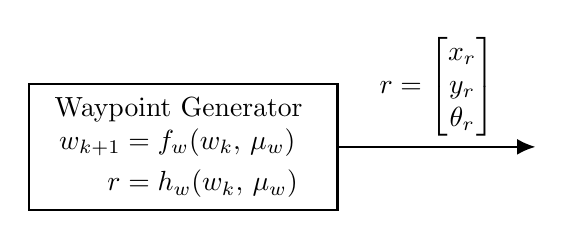
\begin{tikzpicture}[
  block/.style = {draw, thick, minimum height=3em, minimum width=6em, align=center},
  arrow/.style = {thick, -{Latex[width=2mm]}},
  node distance=2.5cm and 2.5cm
]

  % Waypoint Generator
  \node[block] (waypoint) {
    \begin{tabular}{c}
            Waypoint Generator \\
      $\begin{aligned}
      w_{k+1} &= f_w(w_k,\,\mu_w) \\
      r &= h_w(w_k,\,\mu_{w})
       \end{aligned}$
    \end{tabular}
  };


  \draw[arrow] (waypoint.east) -- ++(2.5,0) node[midway,above] {$r = \begin{bmatrix} x_r \\ y_r \\ \theta_r \end{bmatrix}$};


\end{tikzpicture}
\end{document}
